
\documentclass[12pt]{article}


%%% PACKAGES

\usepackage[pdftex]{graphicx}

\usepackage{hyperref}
\usepackage{bibentry} %to use intext full bibliography entries instead of citations.  You will need a separate BibTex database for this to work.  See http://cst.usc.edu/services/tel/grants/legrants.html for details on this package.
\usepackage{booktabs} % for much better looking tables
\usepackage{array} % for better arrays (eg matrices) in maths
\usepackage{paralist} % very flexible & customisable lists (eg. enumerate/itemize, etc.)
%\usepackage{verbatim} % adds environment for commenting out blocks of text & for better verbatim
%\usepackage{subfigure} % make it possible to include more than one captioned figure/table in a single float

\usepackage{caption}

\usepackage{color}

%%% PAGE DIMENSIONS
\usepackage{geometry} % to change the page dimensions. Read ftp://ftp.tex.ac.uk/tex-archive/macros/latex/contrib/geometry/geometry.pdf for detailed page layout information 
\geometry{margin=1in} % for example, change the margins to 1 inches all round
%\geometry{landscape} % set up the page for landscape
% 

%%% HEADERS & FOOTERS
\usepackage{fancyhdr} % This should be set AFTER setting up the page geometry
\pagestyle{fancy} % options: empty , plain , fancy
\renewcommand{\headrulewidth}{0.4pt} % customise the layout...
%\lhead{}\chead{}\rhead{}
%\lfoot{}\cfoot{\thepage}\rfoot{}

%\rfoot{\footnotesize SIR 330}
\rhead{\footnotesize BME 3300 Lab 3}
\renewcommand\footrulewidth{0pt}

\usepackage{enumitem}
%%% SECTION TITLE APPEARANCE
%\usepackage{sectsty}
%\allsectionsfont{\sffamily\mdseries\upshape} % (See the fntguide.pdf for font help)
% (This matches ConTeXt defaults)


%% END Article customise

%%% BEGIN DOCUMENT


\begin{document}


\thispagestyle{plain} %alternatively specify empty to get no footer on first page.  This is part of the fancyhdr package


\nobibliography{MasterBib} %this specifies the BibTex directory that stores your desired bibliography entries.  It has to come before any \bibentry lines are invoked

\bibliographystyle{apalike} %be careful here, there is only a few styles that will run


%\tableofcontents
\begin{center}
\bigskip

\textbf{BME 3300 Lab 3: Electrocardiograms} \medskip

\end{center}

\bigskip
This lab addresses the three fundamental parts of an ECG amplifier: the buffers, the differential amplifier, and signal filtering system.
\vspace{-0.25cm}
\begin{figure}[!h]
\begin{center}
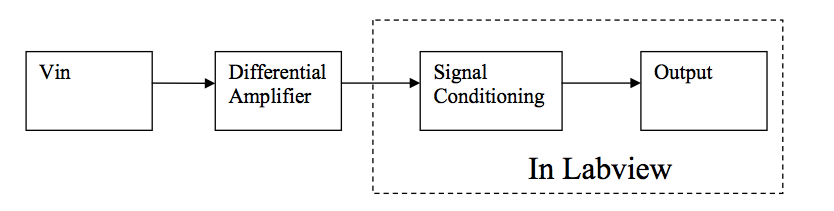
\includegraphics[width=0.85\textwidth,trim=0 0 0 0,clip=false]{figures/flowchart.png}
%\caption{Electrical schematic of electret insides (except for the resistor - that you will add on).
%Image from www.openmusiclabs.com.}
%\label{fig:4}
\end{center}
\end{figure}
\vspace{-1.5cm}
\subsection*{Part 1. The Differential Amplifier}
The key process to the differential amplifier is the CMRR. 
Build the circuit below on a breadboard. 
Use the 356N op-amp for this circuit. 
Use the dual op-amp 412CN for the buffers later. 
Look at the data sheet to see the pin-out for the op-amp. 
These op-amps run off of $\pm$15V. 
To get this from your power supply, first set the tracking on the power supply to ``Series.'' 
Then without anything connected, turn the power supply on, set both switched on the display to ``Volt'', 
turn both ``Current'' knobs fully clockwise, and turn the right ÒVoltageÓ knob until 15.0 is displayed on both displays. 
Do not use the green ``GND'' connections on these power supplies, these connect to chassis ground and will not conduct any current. 
To make a $\pm$15 V supply, the red + terminal from the left side must be attached to the black -- terminal on the right. 
Then -15 V will be on the left terminal, ground in the middle, and +15 V on the right terminal. 
Connect the power leads to the vertical blue and red power busses on the breadboard.

\begin{figure}[!h]
\begin{center}
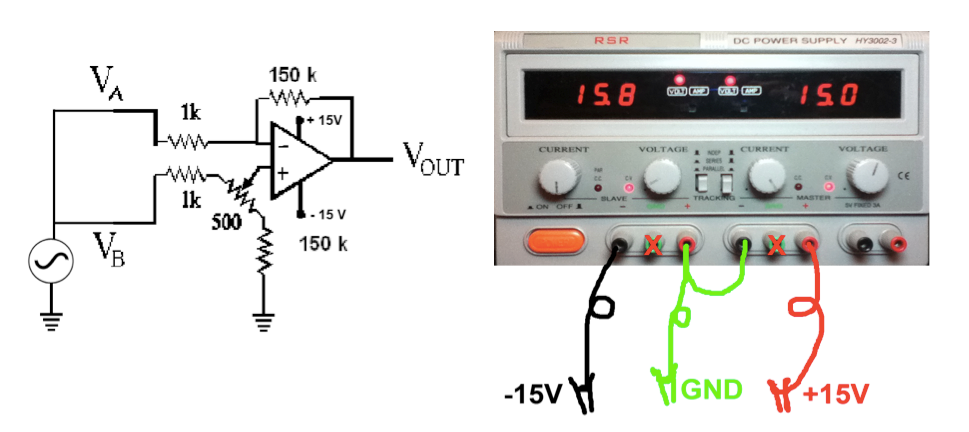
\includegraphics[width=\textwidth,trim=0 0 0 0,clip=false]{figures/circuitandps.png}
%\caption{Electrical schematic of electret insides (except for the resistor - that you will add on).
%Image from www.openmusiclabs.com.}
%\label{fig:4}
\end{center}
\end{figure}

\begin{itemize}
\item Connect a 5 V 60 Hz signal to BOTH $V_A$ and $V_B$. Adjust the potentiometer until $V_{out}$ is a minimum.
\item Note that the potentiometer is just a variable voltage divider. 
The middle pin goes to the non-inverting pin of the op amp and the outer legs are similar to legs that would come out of a normal resistor. 
Use the screw at the end to adjust the resistance at the middle pin. 
What kind of device would you have if you only connected one outer leg and the middle leg into a circuit?
\end{itemize}

\noindent {\textbf{Outputs}}
\begin{itemize}
\item \textbf{Calculate your DMG for this circuit.}
\item \textbf{Since your DMG is 150, determine the CMRR for this circuit.}
\end{itemize}

\subsection*{Part 2. The Buffers}
\begin{itemize}
\item Add two buffers to the circuit above.
\item Put the input signal on both buffer inputs and measure $V_{out}$. 
You may want to tweak the pot again to minimize $V_{out}$.
\end{itemize}

\begin{figure}[!h]
\begin{center}
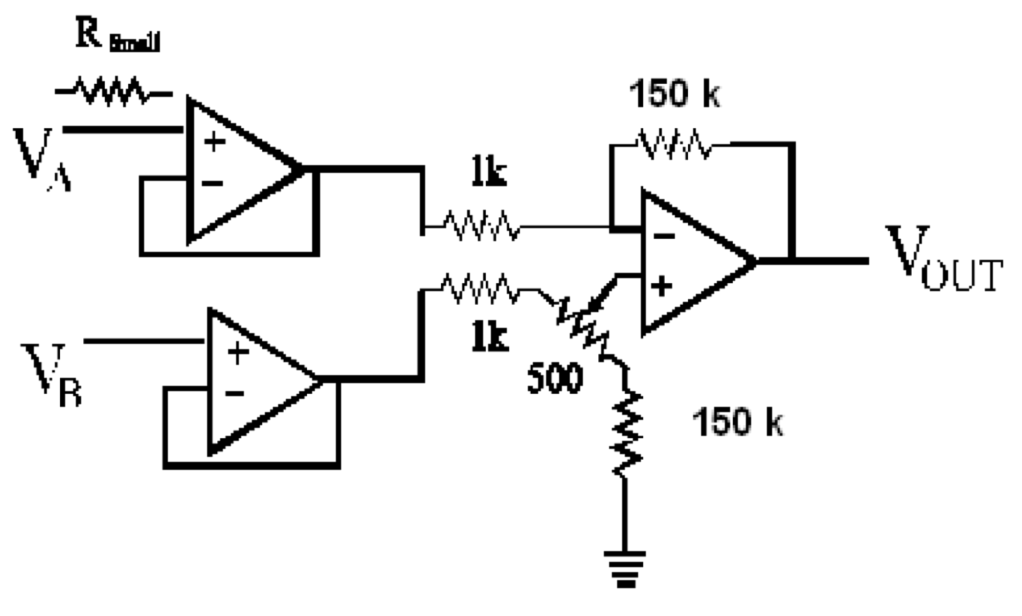
\includegraphics[width=0.5\textwidth,trim=0 0 0 0,clip=false]{figures/circuitwithbuffers.png}
%\caption{Electrical schematic of electret insides (except for the resistor - that you will add on).
%Image from www.openmusiclabs.com.}
%\label{fig:4}
\end{center}
\end{figure}

\noindent {\textbf{Output: Determine the new CMRR.}}

\begin{itemize}
\item Ground the $V_A$ input and apply a small 60 Hz (No DC!) signal to $V_B$. 
Look carefully at $V_{out}$. 
Is there a DC component? 
If so, where is it coming from?
How could you get rid of it, if you wanted to, in the circuit? You will actually remove it after sampling in LabView.
\item Hook up electrode leads to one group member using the left and right wrists, and left ankle. 
For the time being use the left wrist as the positive input, right wrist as the negative input, and the left ankle as ground. 
Later, you may find that you can get a better signal by placing the positive and negative pads on your group member's chest, above and below the heart.
\item Hook up the circuit to the oscilloscope. 
Can you see the ECG signal? 
If not, what could be causing the problem?
\end{itemize}

\subsection*{Part 3. Labview}
\begin{itemize}
\item Start up LabView.
\item Using the DAQ assistant, set LabView to measure $V_{out}$ from the circuit you built. 
Have the DAQ assistant measure 5000 samples at 1000 Hz, measuring continuously.
\item Create a filter that reduces the DC component of the wave (you must choose the filter type...but
choose wisely) and show waveform graph and its Fourier graph.
	\begin{itemize}
		\item To place a filter, right click in the white space of the block diagram and hover over express, then signal analysis, then click on filter. Click again to place the filter where you like.
		\item Right click on the filter and go to properties to change filter type and cutoff frequency.
		\item Right click on the arrow for ``Filtered Signal'' and select create $\rightarrow$ graph indicator. In its
properties, go to the scales tab and tell it so show only from 0 to 5 sec. of the waveform.
		\item To place a Fourier graph, right click on the white space and go to analysis, then spectral
measurements. In properties, make sure that the spectral measurement is set to power spectrum. Be sure to wire the signal in to the proper input and create a graph indicator the same way as before. In the graph's properties show only up to 150 Hz.
	\end{itemize}
\end{itemize}
{\textbf{Output: What are the two frequencies that seem to have the highest level of noise? Why?}}

\begin{itemize}
\item Create another filter in series that eliminates the noise seen in the first Fourier analysis (again, you must choose the filter type). Once again show waveform graph and its Fourier graph.
\item Tweak cutoff frequencies until a clean ECG signal is visible.
\end{itemize}

\noindent {\textbf{Output: Take a screenshot of the three waveforms and their Fourier transforms.}}

\begin{itemize}
\item Now swap the inputs on your breadboard so that you measure the difference between your right wrist and left ankle, with the left wrist as ground. Do you see any difference in the filtered signal? 
\end{itemize}

\noindent {\textbf{Output: Take a screenshot similar to previous one.}}

\begin{itemize}
\item  Again, swap the inputs so that you measure across left wrist and left ankle with right wrist grounded. 
Do you see any difference in the filtered signal?  
Also, which configuration gives you a better p-wave? Why?
\end{itemize}

\noindent {\textbf{Output: Take a screenshot similar to previous ones.}}

\subsection*{Part 4: Importance of the Buffers}
\begin{itemize}
	\item Using the circuit you built and the filters you have created in LabView, remove the buffers and note the change.
\end{itemize}

\noindent {\textbf{Output: Show filtered data with buffers removed. What causes the drastic changes in signal?}}

\end{document} 